%\documentclass[prl,showpacs,amssymb,floatfix,twocolumn]{revtex4-1}
\documentclass[prl,showpacs,amssymb,floatfix]{revtex4-1}
\usepackage{amsmath}
%\bibliographystyle{apsrev}
\usepackage{graphicx}% Include figure files
\usepackage{epsfig}% Include figure files
\usepackage{dcolumn}% Align table columns on decimal point
\usepackage{bm}% bold math
\usepackage{times}
\usepackage{epstopdf}



\begin{document}
\title{KPZ 4D}
\author{Andrea Pagnani$^1$, Giorgio Parisi$^2$}

\affiliation{$^1$ Human Genetics Foundation (HuGeF), Via Nizza 52, I-10126, Turin, Italy\\$^2$ Dipartimento di Fisica, INFN - Sezione di Roma 1, CNR-IPCF UOS Roma, Universit\`a ``La Sapienza'', P.le Aldo Moro 2, I-00185 Roma, Italy} 


\begin{abstract}
  We consider the RSOS discrete surface evolution in 4D.
\end{abstract}
\pacs{02.50.Ey, 05.70.Ln, 64.60.Ht, 68.35.Fx}


\maketitle 

The Kardar-Parisi-Zhang (KPZ) \cite{KPZ86} equation is possibly the
simplest, most studied, and yet not fully understood, model for
out-of-equilibrium surface growth. The equation describes the time
evolution of the height $h({\mathbf r}, t)$ of an interface above a
$d-$dimensional substrate:
\begin{equation}
\label{eq:KPZ}
\partial_t h({\mathbf r}, t) = \nu {\vec \nabla}^2 h({\mathbf r}, t) +
\frac \lambda 2 | {\vec \nabla}h({\mathbf r}, t)|^2 +\eta({\mathbf r}, t) \, ,
\end{equation}
where $\nu$ is the diffusion coefficient, $\lambda$ is the strength of
the non-linear growth rate term which is responsible for the $h
\rightarrow -h$ symmetry breaking with respect to the growing
direction, and $\eta({\mathbf r},t)$ is a Gaussian white noise of
variance (amplitude) $D$:
\begin{equation}
\label{eq:noise}
\langle \eta \rangle = 0 \,\,\,\,\,\,,\,\,\,\,\,\,
\langle \eta({\mathbf r},t) \eta({\mathbf r}',t') \rangle 
= 2D \delta^d({\mathbf r} - {\mathbf r}')
\delta(t-t')\,\,. 
\end{equation}

The KPZ equation describe many relevant growth processes, such as the
Eden model, ballistic deposition, interface growth in disordered
medium. It is also related to many other physical phenomena apparently
unrelated to surface growth, such as Burgers turbulence, dynamics
directed polymers in random media, dissipative transport in the
driven-diffusion equation \cite{FamilyVicsekBook, *BarabasiBook}.

The scaling properties of the height's fluctuations $w_2(L,t) =
\langle h^2 ({\mathbf r}, t) \rangle_{\mathbf r} - \langle h ({\mathbf
  r}, t) \rangle^2_{\mathbf r}$ (with the notation $\langle \dots
\rangle_{\mathbf r}$ we indicate a spatial average over a macroscopic
box of linear size $L$ over the $d-$dimensional substrate)
characterize the universality class of the model. More precisely, for
a system of size $L$, $w_2(L,t) \sim L^{2 \chi} f(t/L^z)$
\cite{FamilyVicsekBook, *BarabasiBook}, where the scaling function is
such that $f(x) \rightarrow \mathrm{const}$ for $x \rightarrow \infty$
and $f(x) \sim x^{2\chi/z}$ for $x \rightarrow 0$. The peculiar
extremal behavior of $f$ imply that $w_2(L,t) \sim L^{2\chi}$ for $t
\gg L^z$ and $w_2(L,t)\sim t^{2 \chi/z}$ for $t \ll L^z$. Due to an
infinitesimal tilt symmetry of Eq.~(\ref{eq:KPZ}) ($h\rightarrow h+{\mathbf r
}\cdot{\boldsymbol \epsilon}$, ${\mathbf r} \rightarrow {\mathbf r} -
\lambda t {\boldsymbol \epsilon} $), the two critical exponents are
related by the scaling relation $\chi + z = 2$, which is believed to
be valid at any dimension $d$.

A complete understanding of Eq.~(\ref{eq:KPZ}), and in particular the
determination of the two critical exponents $\chi,z$ for any spatial
dimension $d>1$ (at $d=1$ a fluctuation-dissipation theorem
leads to the exact result $\chi = 1/2$, $z=3/2$) , turns out to be
extremely difficult for two main reasons: (i) we are dealing with an
intrinsically out-of-equilibrium phenomenon where the standard
equilibrium toolbox must be used with care, (ii) perturbative
renormalization schemes are not adequate for describing the strong
coupling regime ({\em i.e.}~where the parameter $\lambda$ is
relevant). Among the unsolved theoretical issues related with
Eq.~(\ref{eq:KPZ}), that of the existence of an upper critical
dimension $d_u$, {\em i.e.} the substrate dimensionality $d$ above
which the fluctuation of the model become irrelevant ($\chi = 0$), is
among the most controversial ones. The determination of $d_u$ would be
a most relevant achievement, since, as customary in equilibrium
critical phenomena, its knowledge constitutes the first step for a
controlled perturbative expansion around it. The quest for $d_u$ has
been around for more than twenty years
\cite{Halpin-Healy1990,Cook-Derrida1990,
  Schwartz-Edwards1998,Bouchaud-Cates1993,*Bouchaud-Cates-Errata1993,
  DMKB1994,*MBDMBC95, Tu1994, ColaioriMoore2001, Laessig1995,
  *Laessig-Kinzelbach1997, Frogedby2006, CCDW2010, KK1989, *WK1987,
  *TLFWD1992, *Nissila1993,NOIKPZ2001,*NOIKPZ2002, CMP1998,
  *CGMMP1998,*CMMP1999} and the different predictions range from $d_u
\approx 2.8$ to $d_u = \infty$. Analytical estimates using the
mode-coupling theory which yeald exact results in $d=1$
\cite{HwaFrey1991,*FTUH1996}, when extended to higher dimensions, seem
to hint for a $d_u = 4$ under different self-consistency schemes
\cite{Schwartz-Edwards1998,Bouchaud-Cates1993,*Bouchaud-Cates-Errata1993,
  DMKB1994,*MBDMBC95,Tu1994, ColaioriMoore2001}. The same value for
$d_u$ is also supported by different field-theoretic approaches
\cite{Halpin-Healy1990,
  Laessig1995,*Laessig-Kinzelbach1997,Frogedby2006, CCDW2010}.

At odd with what predicted by the previously mentioned field-theoretic
approaches, both direct numerical integration of KPZ equation
\cite{Moser1991}, and simulation of systems belonging to the KPZ
universality class \cite{ KK1989,
  *WK1987,*TLFWD1992,*Nissila1993,NOIKPZ2001,*NOIKPZ2002,Perlsman-Havlin2006,
  *Schwartz-Perlsman2011,KellingOrdor2011} indicate that $d_u > 4$,
while the real-space renormalization group approach \cite{ CMP1998,
  *CGMMP1998,*CMMP1999} predicts $d_u = \infty$.

Such a long standing controversy is the consequence of the
difficulties inherent to both analytical and numerical
approaches. Most of the assumptions made on the functional structure
of the sought solution in the different field-theoretic analysis, as
well as the approximations made in the mode-coupling theories are, in
general, not completely under control. On the numerical side the most
severe problem is due to the fact that simulations in high spatial
dimensions $d \geq 4$ are computationally very heavy, and the systems
under analysis must be limited in size. As a consequence, the
different fitting procedures in order to yield reliable estimates of
the critical exponents, must deal with controlled finite-size scaling
procedures. Under this perspective, particularly relevant is the
observation that for lattice models in the KPZ universality class, a
controlled asymptotic regime is achieved only when typical scale of
the fluctuations is larger than the lattice spacing used in the
simulations or, more precisely, for $w_2 > 1$
\cite{ColaioriMoore2001}.

\begin{eqnarray}
\label{eq:fit}
w_2  &=& A_2 L^{2\chi}( 1 + B_2 L^{-\omega})\nonumber\\
w_3  &=& A_3 L^{3\chi}( 1 + B_3 L^{-\omega})\\
w_4  &=& A_4 L^{4\chi}( 1 + B_4 L^{-\omega})\nonumber
\end{eqnarray}
We simulate $4-$dimensional lattices of volume $V = L^4$. 



\begin{itemize}
\item Multi-surface coding
\item Multi-spin coding of the lattice.
\end{itemize}


\begin{figure}[t]
\begin{center}
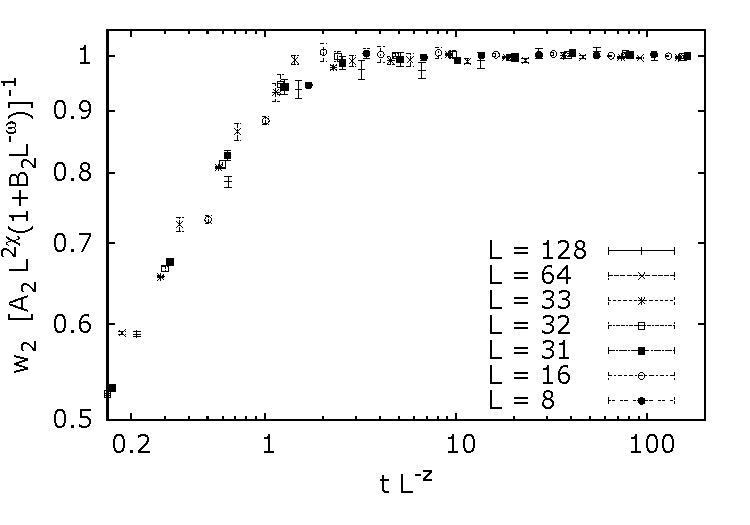
\includegraphics[width=8.5cm]{scalingplot}
\end{center}
\caption{Scaling plot}
\end{figure}




\begin{table}[htb]
\begin{tabular}{|*{5}{c|}}
\hline
 $L$ & mc-sweeps  & samples & type & time (h.)\\
\hline
\hline
8 & 524000 & 1024 & MS & 4 \\
\hline
16 & 524000 & 256 & MS & 6 \\
\hline
31 & 524000 &  256 & MS &121 \\
\hline
32 & 524000 & 256 & MS & 139 \\
\hline
33 & 524000 & 256 & MS & 158 \\
\hline
64 & 131000 & 512 & MS  & 5376 \\
\hline
128 & 512000 & 32 & ML & 7680 \\
\hline
256 & 130000 & 3 & ML & 504 \\
\hline
\end{tabular}
\protect\caption{In this table we display the lattice linear size $L$
  the number of montecarlo sweeps (full lattice update), the number of
  samples and the simulation type (MS = multi-surface coding, ML =
  lattice multi-spin coding), overall computational time in hours}
\label{tab:simulpara}
\end{table}

\begin{table}[htb]
\begin{tabular}{|*{9}{l|}}
\hline
  & $\chi$ & $\omega$ & $A_2$ & $B_2$  & $A_3$ &  $B_3$ & $A_4$ & $B_4$ \\
\hline
\hline
NEW & 0.2532(5)  & 1.14(5) & 0.1720(5)& 0.37(3)& 0.0321(2)& -1.09(8) & 0.1012(6)&  0.36(4) 
\\
\hline
OLD &  0.255(3) &0.98(9) & 0.170(1)& 0.37(3) & 0.0321(2) & -0.7(1) & 0.100(1) & 0.46(4) 
\\
\hline
\end{tabular}
\protect\caption{In this table we display the best fit values together
with their statistical error of the parameters defined in
Eq.~(\ref{eq:fit}). The first row refers to the actual data presented
in this work, the second to the values in \cite{NOIKPZ2001}}
\label{tab:fitpara}
\end{table}








%\bibliographystyle{unsrt}
\bibliography{kpz4d}

\end{document}
